\documentclass[dvisvgm,border=2pt]{standalone}
% Shared by every figure. Two colours only: black becomes the text colour of
% whatever theme the app is in, and `accent` becomes the brand — see
% scripts/build-figures.mjs. Everything else is done with opacity.
\usepackage{amsmath}
\usepackage{amssymb}
\usepackage{tikz}
\usepackage{pgfplots}
\pgfplotsset{compat=1.18}
\usetikzlibrary{arrows.meta,positioning,calc,backgrounds,fit,patterns.meta}
\definecolor{accent}{RGB}{255,0,255}
\pgfplotsset{
  every axis/.append style={
    axis lines=left,
    axis line style={draw opacity=0.35},
    tick style={draw opacity=0.35},
    tick label style={font=\scriptsize,opacity=0.7},
    label style={font=\scriptsize,opacity=0.7},
    legend style={draw=none,fill=none,font=\scriptsize},
    every axis plot/.append style={line width=0.7pt},
  },
}
\tikzset{
  every picture/.style={font=\scriptsize},
  faint/.style={opacity=0.3},
  quiet/.style={opacity=0.55},
  box/.style={draw,opacity=0.35,rounded corners=2pt,inner sep=4pt},
  hot/.style={accent},
}

\begin{document}
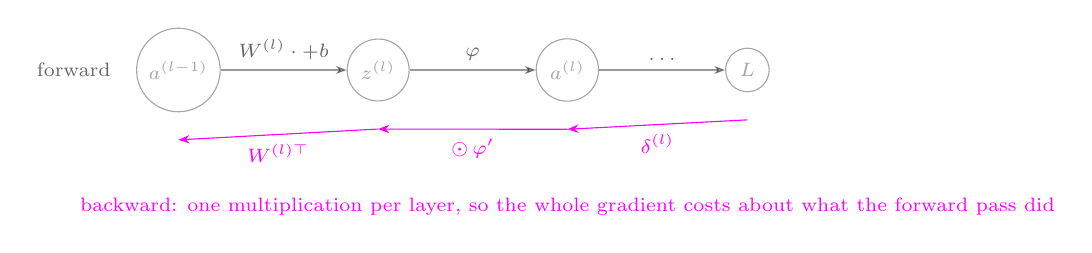
\begin{tikzpicture}[every node/.style={font=\scriptsize},node distance=16mm]
  \node[circle,draw,opacity=0.35,inner sep=3pt] (x) {$a^{(l-1)}$};
  \node[circle,draw,opacity=0.35,inner sep=3pt,right=of x] (z) {$z^{(l)}$};
  \node[circle,draw,opacity=0.35,inner sep=3pt,right=of z] (a) {$a^{(l)}$};
  \node[circle,draw,opacity=0.35,inner sep=3pt,right=of a] (L) {$L$};
  \draw[opacity=0.4,-{Stealth[length=4pt]}] (x) -- node[above,opacity=0.6]{$W^{(l)}\cdot+b$} (z);
  \draw[opacity=0.4,-{Stealth[length=4pt]}] (z) -- node[above,opacity=0.6]{$\varphi$} (a);
  \draw[opacity=0.4,-{Stealth[length=4pt]}] (a) -- node[above,opacity=0.6]{$\ldots$} (L);
  \node[opacity=0.6,anchor=east] at ($(x.west)+(-0.2,0)$) {forward};
  \draw[accent,-{Stealth[length=4pt]}] ($(L.south)+(0,-0.35)$) -- ($(a.south)+(0,-0.35)$)
    node[midway,below,accent]{$\delta^{(l)}$};
  \draw[accent,-{Stealth[length=4pt]}] ($(a.south)+(0,-0.35)$) -- ($(z.south)+(0,-0.35)$)
    node[midway,below,accent]{$\odot\,\varphi'$};
  \draw[accent,-{Stealth[length=4pt]}] ($(z.south)+(0,-0.35)$) -- ($(x.south)+(0,-0.35)$)
    node[midway,below,accent]{$W^{(l)\top}$};
  \node[accent,anchor=north,align=center] at ($(a.south)+(0,-1.1)$)
    {backward: one multiplication per layer, so the whole gradient\ costs about what the forward pass did};
\end{tikzpicture}
\end{document}
